\documentclass{article}

% Recommended, but optional, packages for figures and better typesetting:
\usepackage{microtype}
\usepackage{graphicx}
\usepackage{subfigure}
\usepackage{booktabs} % for professional tables

% hyperref makes hyperlinks in the resulting PDF.
% If your build breaks (sometimes temporarily if a hyperlink spans a page)
% please comment out the following usepackage line and replace
% \usepackage{icml2018} with \usepackage[nohyperref]{icml2018} above.
\usepackage{hyperref}

% Attempt to make hyperref and algorithmic work together better:
\newcommand{\theHalgorithm}{\arabic{algorithm}}

% Use the following line for the initial blind version submitted for review:
%\usepackage{icml2018}

% If accepted, instead use the following line for the camera-ready submission:
\usepackage[accepted]{icml2018}

% The \icmltitle you define below is probably too long as a header.
% Therefore, a short form for the running title is supplied here:
%\icmltitlerunning{}

\begin{document}

\twocolumn[
\icmltitle{Genetic Algorithm for Knapsack Problem}

% It is OKAY to include author information, even for blind
% submissions: the style file will automatically remove it for you
% unless you've provided the [accepted] option to the icml2018
% package.

% List of affiliations: The first argument should be a (short)
% identifier you will use later to specify author affiliations
% Academic affiliations should list Department, University, City, Region, Country
% Industry affiliations should list Company, City, Region, Country

% You can specify symbols, otherwise they are numbered in order.
% Ideally, you should not use this facility. Affiliations will be numbered
% in order of appearance and this is the preferred way.
\icmlsetsymbol{equal}{*}

\begin{icmlauthorlist}
    \icmlauthor{Ond\v{r}ej Podsztavek}{fit}
\end{icmlauthorlist}

\icmlaffiliation{fit}{
    Faculty of Information Technology, Czech Technical University in Prague,
    Prague, Czech Republic
}

\icmlcorrespondingauthor{Ond\v{r}ej Podsztavek}{podszond@fit.cvut.cz}

% You may provide any keywords that you
% find helpful for describing your paper; these are used to populate
% the "keywords" metadata in the PDF but will not be shown in the document
\icmlkeywords{genetic algorithm, knapsack problem}

\vskip 0.3in
]

% this must go after the closing bracket ] following \twocolumn[ ...

% This command actually creates the footnote in the first column
% listing the affiliations and the copyright notice.
% The command takes one argument, which is text to display at the start of the footnote.
% The \icmlEqualContribution command is standard text for equal contribution.
% Remove it (just {}) if you do not need this facility.

\printAffiliationsAndNotice{}  % leave blank if no need to mention equal contribution
%\printAffiliationsAndNotice{\icmlEqualContribution} % otherwise use the standard text.

\begin{abstract}
This work presents a simple genetic algorithm for knapsack problem.
Two fitness function are proposed.
Followed by evaluation of some selection method and parameters setting.
Conclusion is that tournament selection of size 3, cross-over rate 0.6
and mutation rate 0.001 work best for most knapsack problem instances.
\end{abstract}

%\section{Introduction}

\section{0/1 Knapsack Problem}

Given whole number $n$ (number of things),
whole number $M$ (knapsack capacity),
finite set $W = \{w_1, w_2, \dots , w_n\}$ (things' weights),
finite set $C = \{c_1, c_2, \dots , c_n\}$ (things' cost).
Construct set $X = \{x_1, x_2, \dots , x_n\}$ where all $x_i \in \{0, 1\}$,
so that $w_1 x_1 + w_2 x_2 + \dots + w_n x_n \leq M$
(knapsack is not overloaded)
and expression $c_1 x_1 + c_2 x_2 + \dots + c_n x_n$ is maximal for all such
sets (cost of things in knapsack is maximal).

\section{Genetic Algorithm}

The idea of genetic algorithms is to evolve a population of solutions
to a given problem using operators inspired by natural genetic variation
and natural selection.
\cite{mitchell1996}

There is no rigorous definition of genetic algorithm but most methods
have at least in common populations of chromosomes,
selection according to fitness, crossover to produce new offspring
and random mutation of new offspring.
\cite{mitchell1996}

The term \textit{chromosome} refers to a solution to a problem
which is encoded as a bit string
and can be thought of as points in the search space of solutions.
The \textit{genes} are either single or short blocks bits
that encode a particular element of the solution.
An \textit{allele} is 0 or 1 in bit string.
Mostly genetic algorithms employ \textit{single-chromosome haploid} individuals.
The \textit{genotype} of an individual is the configuration of bits
in its chromosome.
\cite{mitchell1996}

The simplest form of genetic algorithm involves three types of operators.
\textit{Selection} in operator which selects chromosomes in the population for
reproduction.
The fitter the chromosome the more it is likely to be selected.
\textit{Crossover} randomly chooses a position in a chromosome
and exchange the subsequences before and after the position between
two chromosomes to create two new offspring.
\textit{Mutation} randomly flips some bits in a chromosome.
\cite{mitchell1996}

The algorithm processes population of chromosomes successively replacing
one population with another (see algorithm~\ref{alg:ga}).
Genetic algorithm requires a fitness function that assigns a score to
each chromosome in the current population.
The chromosome's fitness depends on how well the chromosome solves given
problem.
\cite{mitchell1996}

\begin{algorithm}[hb]
\caption{Genetic Algorithm~\cite{eiben2003}}
\label{alg:ga}
\begin{algorithmic}
\STATE initialize population with random individuals
\STATE evaluate each individual
\WHILE{terminal condition is not satisfied}
\STATE select parents
\STATE recombine pairs of parents
\STATE mutate the resulting offspring
\STATE evaluate new individuals
\STATE select individuals for next generation
\ENDWHILE
\end{algorithmic}
\end{algorithm}

\section{Implementation}

The implementation is in Python 3.6 programming language
and is based on DEAP framework~\cite{fortin2012}.

Chromosomes representation is straight forward for 1/0 knapsack problem.
A chromosome is represented as Python's list of numbers 0 and 1.
If there is 1 at position $i$ it means that items with weight $w_i$ and $c_i$
is included in knapsack while 0 means that the item is not included.

Two different fitness functions are implemented
because some individual generated by a genetic algorithm might not satisfy
the knapsack constrain.
One with individual correction and second using penalization.

The correction fitness function randomly removes bits with value 1
from an individual until the individual does not overload knapsack.
Then the value of the fitness function is the sum of costs of things
in knapsack.

The fitness function with penalization is the sum of costs of things
in knapsack if not overloaded else it is the negative weight of things
in knapsack.

The skeleton of implemented genetic algorithm is the same as
in algorithm~\ref{alg:ga}.
Population size is fixed through all generation.

In order to stop the evolution of population advantage of
\textit{early stopping} is taken.
This mechanism works based on average fitness of population increase.
If population's average fitness does not increase by a certain amount
during given number of generation the evolution is terminated.

Last commonly used method applied is \textit{elitism}.
This method puts chosen number of elite individuals with best fitness
from previous generation to next generation.

\section{Experiments}

There is many parameters which need to be set in genetic algorithm.
It is impossible to explore them all.
Therefore, a heuristic approach has to be taken.

For purpose of this work firstly fitness function is chosen
from the two candidates.
Parameters are set according to proposition in~\cite{dejong1975}.
Population is of size 100 individuals,
two point crossover with rate 0.6 per pair of parents
and mutation rate is 0.001 per bit.
One elite individual is moved to next generation.
Evolution is stopped if there is no increase by 1 in fitness
value of next 50 average generation's fitness.

\begin{figure}[ht]
\vskip 0.2in
\begin{center}
\centerline{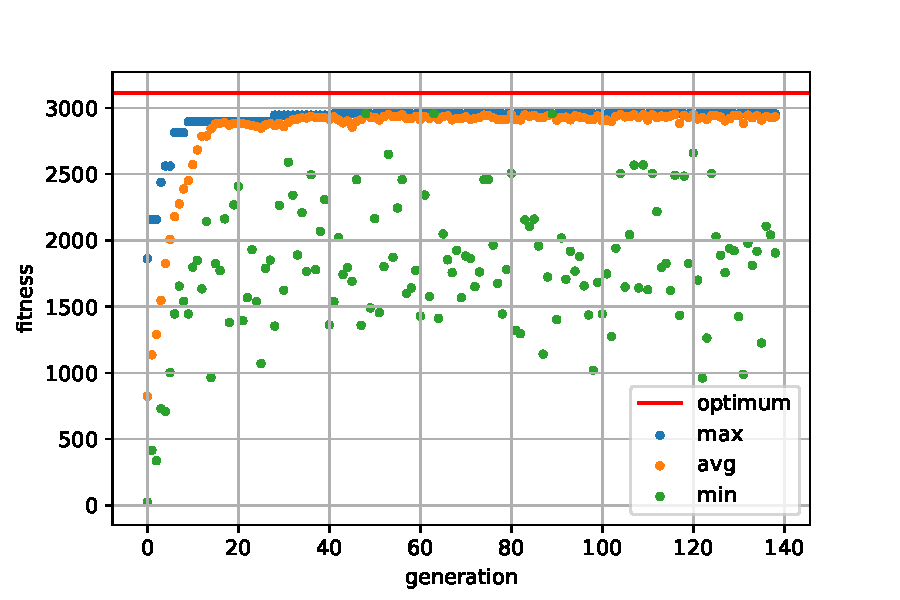
\includegraphics[width=\columnwidth]{evolution}}
\caption{Evolution of population for sample knapsack problem.}
\label{evolution}
\end{center}
\vskip -0.2in
\end{figure}

Experiments were carried out on Intel Core i5-3337U CPU (1.80GHz)
using instances of sizes 32, 50, 75, 100, 150, 200, 500.
There were 500 instances for each size.

\subsection{Fitness Functions}

This work proposed two different fitness functions.
Figure~\ref{fitness} presents their experimental evaluation.
Both fitness functions perform comparably on average
but the maximal relative error is much higher
for fitness function with penalization.
From that its instability can be inferred.

\begin{figure}[ht]
\vskip 0.2in
\begin{center}
\centerline{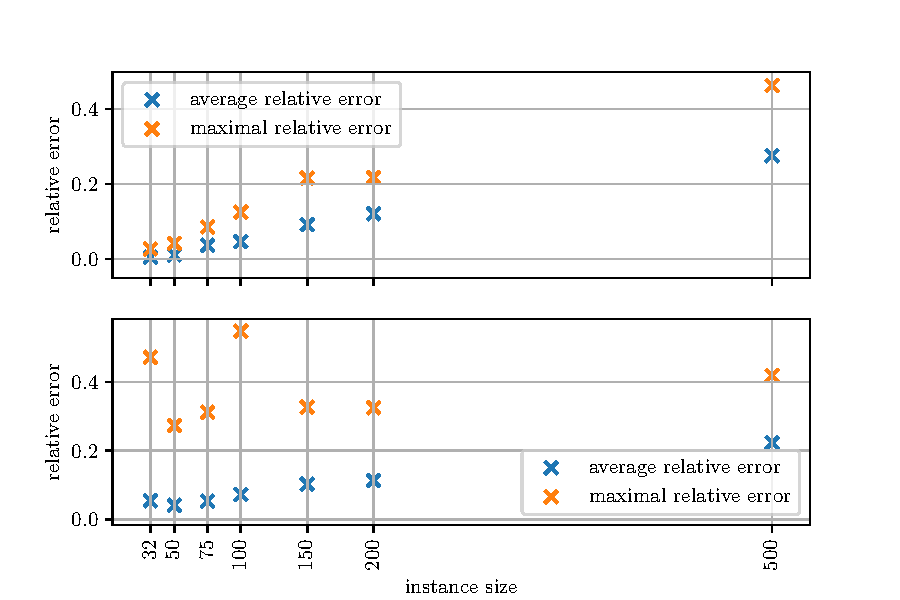
\includegraphics[width=\columnwidth]{fitness}}
\caption{The top plot shows relative error of fitness function with
correction and bottom plot relative error of fitness function with
penalization.}
\label{fitness}
\end{center}
\vskip -0.2in
\end{figure}

Thus, for further experiments fitness function with correction will be used
as it gives better overall performance for different instances.

\subsection{Selection Method}

Selection is important part of a genetic algorithm selecting parents of next
generation.
There are many possible options such as roulette, tournament
or random selection.
This work compares roulette to tournament selections.

Figure~\ref{fitness} shows results for roulette selection
and figure~\ref{tournament} results for tournament selection of size 3.
It is obvious that tournament selection outperforms roulette selection in
most cases.
Only the maximal relative error of some small instances are better for
roulette selection.
For further evaluations tournament of size 3 is used.

\begin{figure}[ht]
\vskip 0.2in
\begin{center}
\centerline{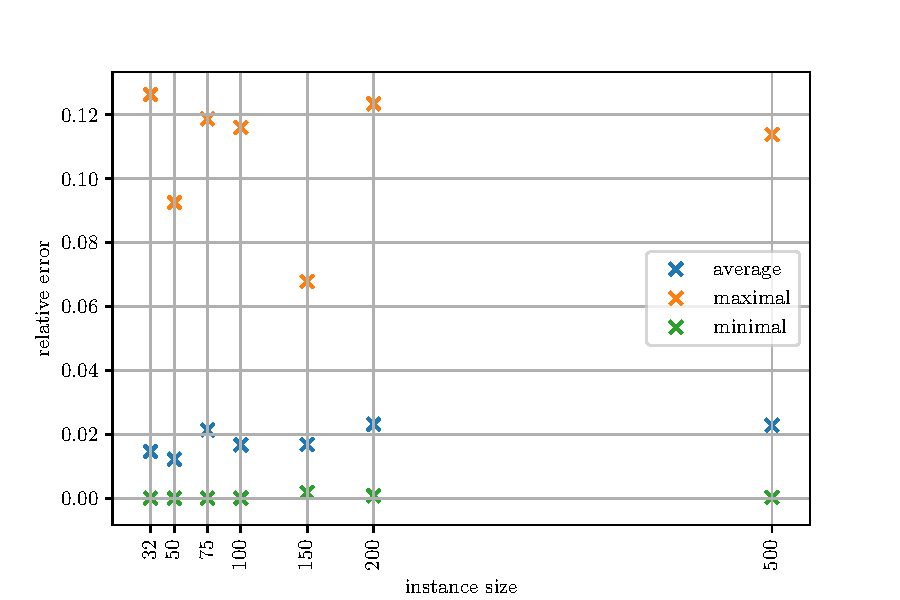
\includegraphics[width=\columnwidth]{tournament}}
\caption{Maximal, average and minimal relative error of tournament selection
of size 3.}
\label{tournament}
\end{center}
\vskip -0.2in
\end{figure}

\subsection{Parameters}

Parameters as crossover and mutation rate are very import in a genetic
algorithm.
In this subsection recommendation from~\cite{schaffer1989} are used.
Population size of 30, crossover rate of 0.95 and mutation rate of 0.01
are tested.

Result is presented in figure~\ref{params}
and unfortunately is worse than with original parameter setting.

\begin{figure}[ht]
\vskip 0.2in
\begin{center}
\centerline{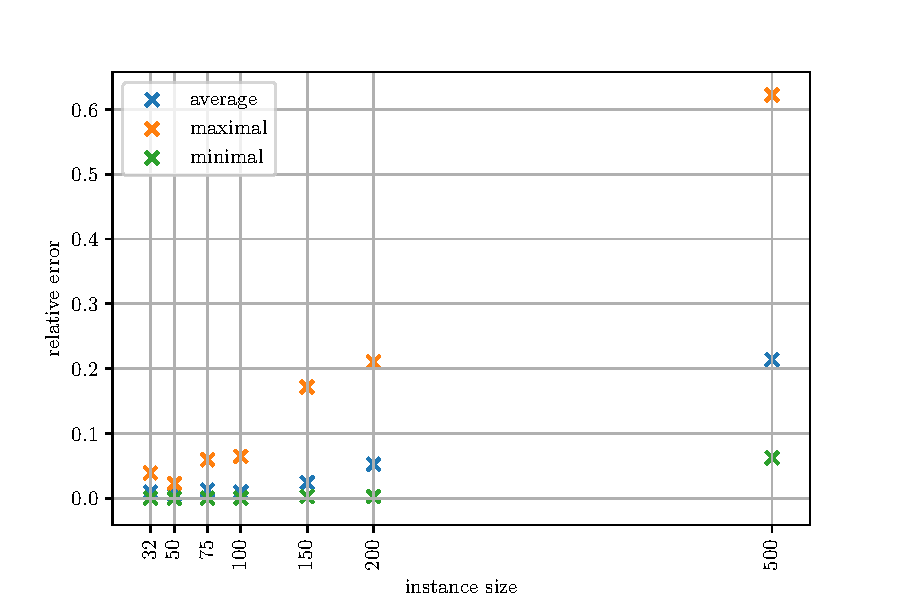
\includegraphics[width=\columnwidth]{params}}
\caption{Relative error for population size 30, crossover rate 0.95
and mutation rate 0.01.}
\label{params}
\end{center}
\vskip -0.2in
\end{figure}

\section{Conclusion}

In conclusion, this work show that a simple genetic algorithm
when correctly parameterized can solve even big instances of knapsack problem
with small relative error around 2\% (see figure~\ref{tournament}).

A concern might be computation time which depends on population size
and instance size (see figure~\ref{time})
but further experiments should be able to reduce it.

\begin{figure}[ht]
\vskip 0.2in
\begin{center}
\centerline{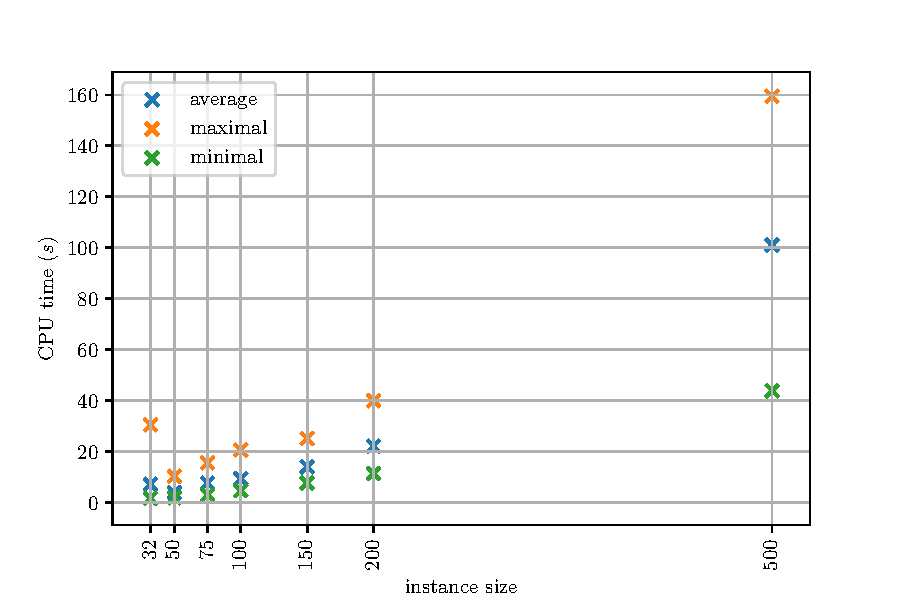
\includegraphics[width=\columnwidth]{time}}
\caption{Dependence of CPU time on instance size for tournament selection
of size 3.}
\label{time}
\end{center}
\vskip -0.2in
\end{figure}

% In the unusual situation where you want a paper to appear in the
% references without citing it in the main text, use \nocite
%\nocite{langley00}

\bibliography{report}
\bibliographystyle{icml2018}

\end{document}

% This document was modified from the file originally made available by
% Pat Langley and Andrea Danyluk for ICML-2K. This version was created
% by Iain Murray in 2018. It was modified from a version from Dan Roy in
% 2017, which was based on a version from Lise Getoor and Tobias
% Scheffer, which was slightly modified from the 2010 version by
% Thorsten Joachims & Johannes Fuernkranz, slightly modified from the
% 2009 version by Kiri Wagstaff and Sam Roweis's 2008 version, which is
% slightly modified from Prasad Tadepalli's 2007 version which is a
% lightly changed version of the previous year's version by Andrew
% Moore, which was in turn edited from those of Kristian Kersting and
% Codrina Lauth. Alex Smola contributed to the algorithmic style files.
